\documentclass{article}

\usepackage{graphicx}
\usepackage{tikz}
\usepackage{tikzsymbols}
\usetikzlibrary{calc,patterns,shapes.geometric}
\pagestyle{empty}
\usepackage[margin=0pt]{geometry}
\geometry{papersize={14in,12in}}

\def\centerarc[#1](#2)(#3:#4:#5){\draw[#1] ($(#2)+({#5*cos(#3)},{#5*sin(#3)})$) arc (#3:#4:#5);}

\begin{document}
	\begin{figure}
		\centering
		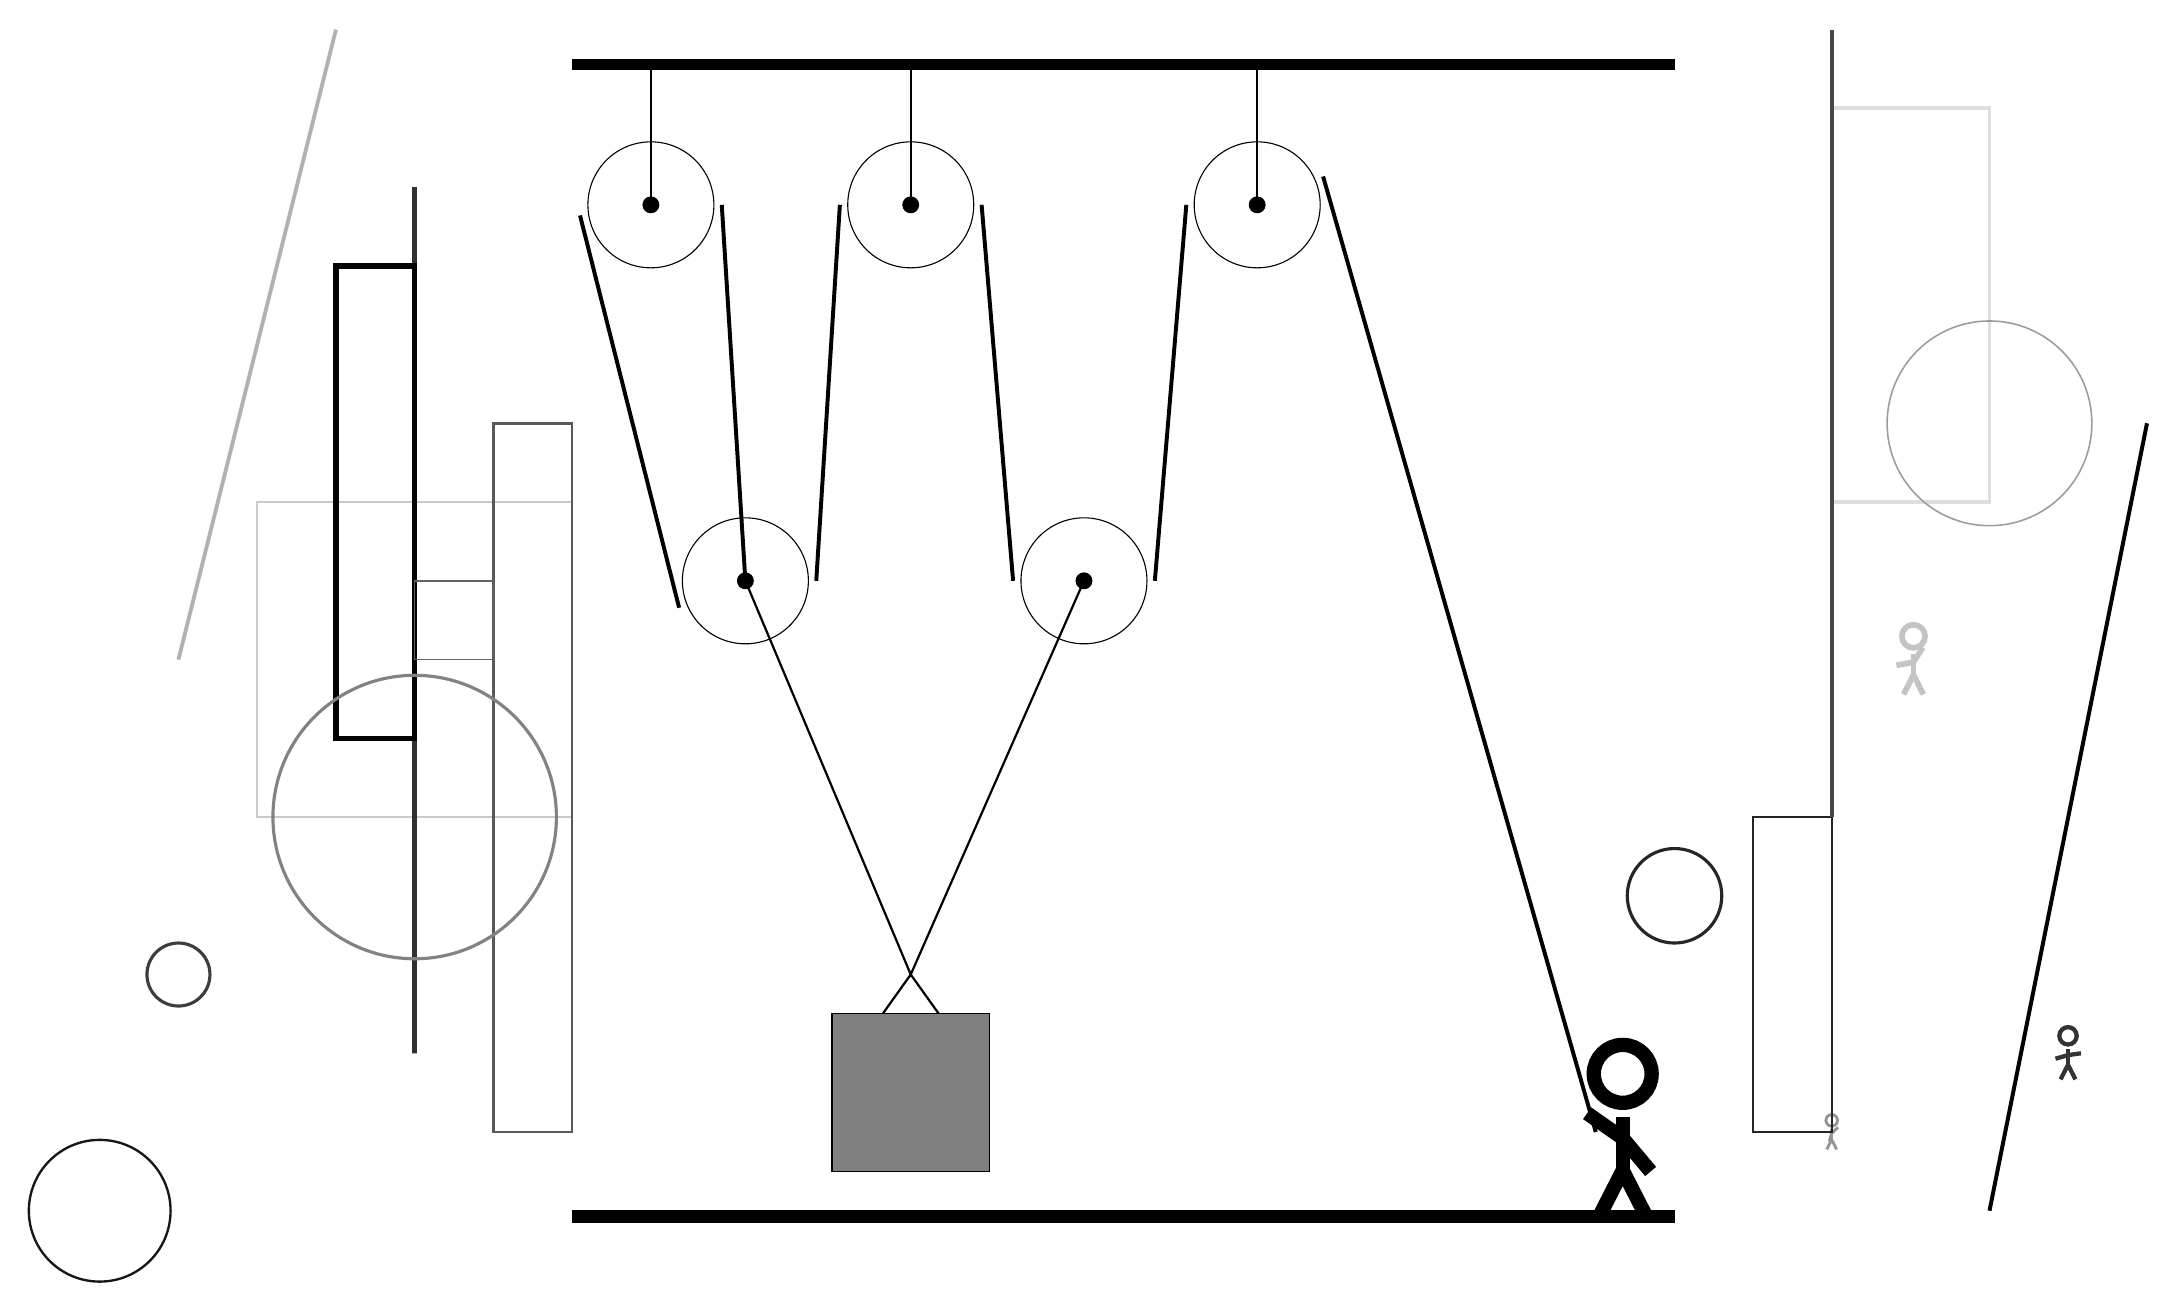
\begin{tikzpicture}
			%%%%% START %%%%%
			
			\draw[fill=black] (-2, 11.5) rectangle (12, 11.625);
			
			\draw (-1, 9.775) circle (0.8);
			\draw[fill=black] (-1, 9.775) circle (0.1);
			\draw[thick] (-1, 9.775) -- (-1, 11.5);
			
			\draw (2.3, 9.775) circle (0.8);
			\draw[fill=black] (2.3, 9.775) circle (0.1);
			\draw[thick] (2.3, 9.775) -- (2.3, 11.5);
			
			\draw (6.7, 9.775) circle (0.8);
			\draw[fill=black] (6.7, 9.775) circle (0.1);
			\draw[thick] (6.7, 9.775) -- (6.7, 11.5);
			
			\draw (0.2, 5) circle (0.8);
			\draw[fill=black] (0.2, 5) circle (0.1);
			
			\draw (4.5, 5) circle (0.8);
			\draw[fill=black] (4.5, 5) circle (0.1);
			
			\draw[thick] (0.2, 5) -- (2.3, 0)  -- (4.5, 5);
			\draw[thick]  (1.8, -0.7) -- (2.3, 0) -- (2.8, -0.7);
			\draw[fill=black!50] (1.3, -0.5) rectangle (3.3, -2.5);
			
			\draw[line width=0.5mm] (0.2, 5) -- (-0.1, 9.775);
			\centerarc[line width=0.5mm](-1, 9.775)(0:200:0.9);
			\draw[line width=0.5mm] (-1.9, 9.64) -- (-0.6415, 4.658);
			\centerarc[line width=0.5mm](0.2, 5)(200:360:0.9);
			\draw[line width=0.5mm](1.1, 5) -- (1.4, 9.775);
			\centerarc[line width=0.5mm](2.3, 9.775)(0:180:0.9);
			\draw[line width=0.5mm] (3.2, 9.775) -- (3.6, 5);
			\centerarc[line width=0.5mm](4.5, 5)(180:360:0.9);
			\draw[line width=0.5mm] (5.4, 5) -- (5.8, 9.775);
			\centerarc[line width=0.5mm](6.7, 9.775)(20:180:0.9);
			\draw[line width=0.5mm](7.537, 10.135)  -- (11, -2);
			
			\node at (11.3, -2) {\Strichmaxerl[10][-35][-50]};
			
			\draw[line width=0.5mm, color=black!13] (14, 6) rectangle (16, 11);
			
			\draw[line width=0.3mm, color=black!21] (-2, 2) rectangle (-6, 6);
			\node[line width=0.4mm, color=black!80] at (17, -1) {\Strichmaxerl[3][16][8]};
			\node[line width=0.4mm, color=black!42] at (14, -2) {\Strichmaxerl[2][73][43]};
			\draw[line width=0.6mm, color=black!81] (-4, -1) rectangle (-4, 10);
			\draw [line width=0.2mm, color=black!39](16, 7) circle (1.3);
			\draw[line width=0.3mm, color=black!86] (13, 2) rectangle (14, -2);
			\node[line width=0.6mm, color=black!23] at (15, 4) {\Strichmaxerl[4][11][57]};
			\draw [line width=0.4mm, color=black!85](12, 1) circle (0.6);
			\draw[line width=0.5mm, color=black!100](16, -3) -- (18, 7);
			\draw [line width=0.4mm, color=black!76](-7, 0) circle (0.4);
			
			\draw[line width=0.3mm, color=black!65] (-2, 7) rectangle (-3, -2);
			\draw[line width=0.5mm, color=black!72](14, 2) -- (14, 12);
			\draw[line width=0.7mm, color=black!99] (-4, 3) rectangle (-5, 9);
			\draw[line width=0.2mm, color=black!61] (-4, 5) rectangle (-3, 4);
			\draw [line width=0.4mm, color=black!49](-4, 2) circle (1.8);
			\draw[line width=0.5mm, color=black!30](-7, 4) -- (-5, 12);
			\draw [line width=0.3mm, color=black!91](-8, -3) circle (0.9);
			
			\draw[fill=black] (-2, -3) rectangle (12, -3.15);
			
			%%%%% END %%%%%
		\end{tikzpicture}
	\end{figure}	
\end{document}